\documentclass[10pt,a4paper]{article}
\usepackage[utf8]{inputenc}
\usepackage[francais]{babel}
\usepackage[T1]{fontenc}
\usepackage{amsmath}
\usepackage{amsfonts}
\usepackage{amssymb}
\usepackage{graphicx}
\usepackage{epstopdf}
\usepackage{fancyhdr}
\pagestyle{fancy}
\usepackage{cite}


\renewcommand{\headrulewidth}{1pt}
\fancyhead[R]{} 
\fancyhead[L]{\textit{\leftmark}}

\addtolength{\hoffset}{-1.5cm}
\addtolength{\textwidth}{3.5cm}

\title{Projet MDI 343 \\
Systèmes de recommandation}
\author{Nicolas Keriven et Jean-Baptiste Alayrac}

\begin{document}
\maketitle

\hrulefill
\vspace{2cm}

% Si on veut mettre un abstract

%\renewcommand{\abstractname}{Résumé}
%\begin{abstract}
%
%
%\end{abstract}

% Figure 
%\begin{center}
%\begin{figure}[ht!]
%\includegraphics[width=\columnwidth]{fig/name.extension}
%\caption{\label{lab} titre}
%\end{figure}
%\end{center}

\newpage
\tableofcontents

\section*{Introduction}
\addcontentsline{toc}{section}{Introduction}
 
\newpage


\section{Présentation du problème et notations}

Le cadre général de la problématique de recommandation est de relier des utilisateurs à des produits. Dans cette partie nous présentons tout d'abord les méthodes les plus utilisées actuellement pour les système de recommandations avant de nous concentrer sur la méthode que nous avons approfondie.

\subsection{Différentes méthodes}

Actuellement, il existe deux principales approches afin de  créer un système de recommandation. La première approche est appelée \textit{content filtering} alors que la seconde est nommée \textit{collaborative filtering}

\subsubsection*{\textit{Content filtering} (ou filtrage par contenu)}

Cette méthode vise à caractériser la nature de chaque utilisateur ainsi que de chaque produit afin d'en dégager un profil le plus précis possible. Pour un utilisateur, cela peut être son pays d'origine, son âge... Pour un produit, par exemple un film, cela peut être son genre, son box-office... Les algorithmes ont alors pour tâche d'associer des profils d'utilisateurs avec des profils de produits. Le projet Music Genome Project, utilisé notamment dans la radio Pandora.com utilise de telles méthodes afin de proposer du contenu aux utilisateurs. Chaque musique est alors caractérisée par des centaines d'attributs assimilable à des "gènes". 


\subsubsection*{\textit{Collaborative filtering} (ou filtrage collaboratif)}

L'autre méthode se base essentiellement sur des avis passés (implicites ou explicites) d'utilisateurs à propos de produits. La méthode de \textit{collaborative filtering} analyse les liens qui existent entre utilisateurs et produits via la connaissance de votes passés afin de proposer de nouvelles associations utilisateur/produit. L'avantage principal de cette méthode par rapport à celle de \textit{content filtering} est qu'ici il n'y a nul besoin de connaître le produit ou les utilisateurs à priori. Par contre cette méthode connait le problème du \textit{cold start}, i.e., elle est incapable de traiter l'arrivée d'un nouveau produit ou d'un nouveau utilisateur. Afin de la faire fonctionner il faut posséder un nombre déjà conséquents d'avis de chaque utilisateurs et pour chaque produits.

Dans ce contexte de \textit{collaborative filtering} il existe à nouveau deux principales méthodes. La première est connue sous le nom de \textit{neighborhood method}, la deuxième se concentre autour de \textit{latent factor models}.

\begin{figure}[ht!]
\begin{center}
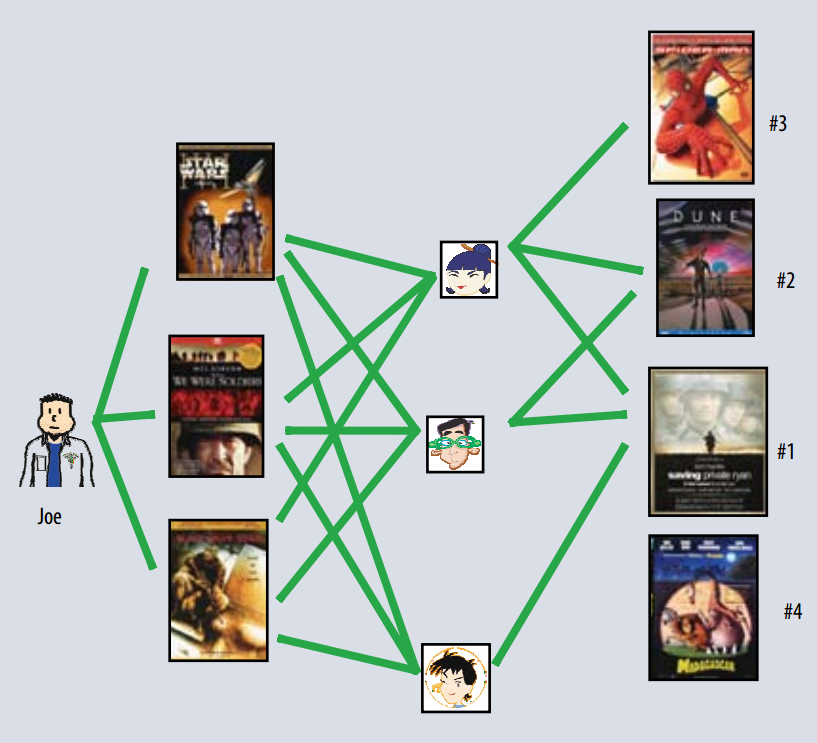
\includegraphics[height=5cm]{fig/neighboor_representation.png}
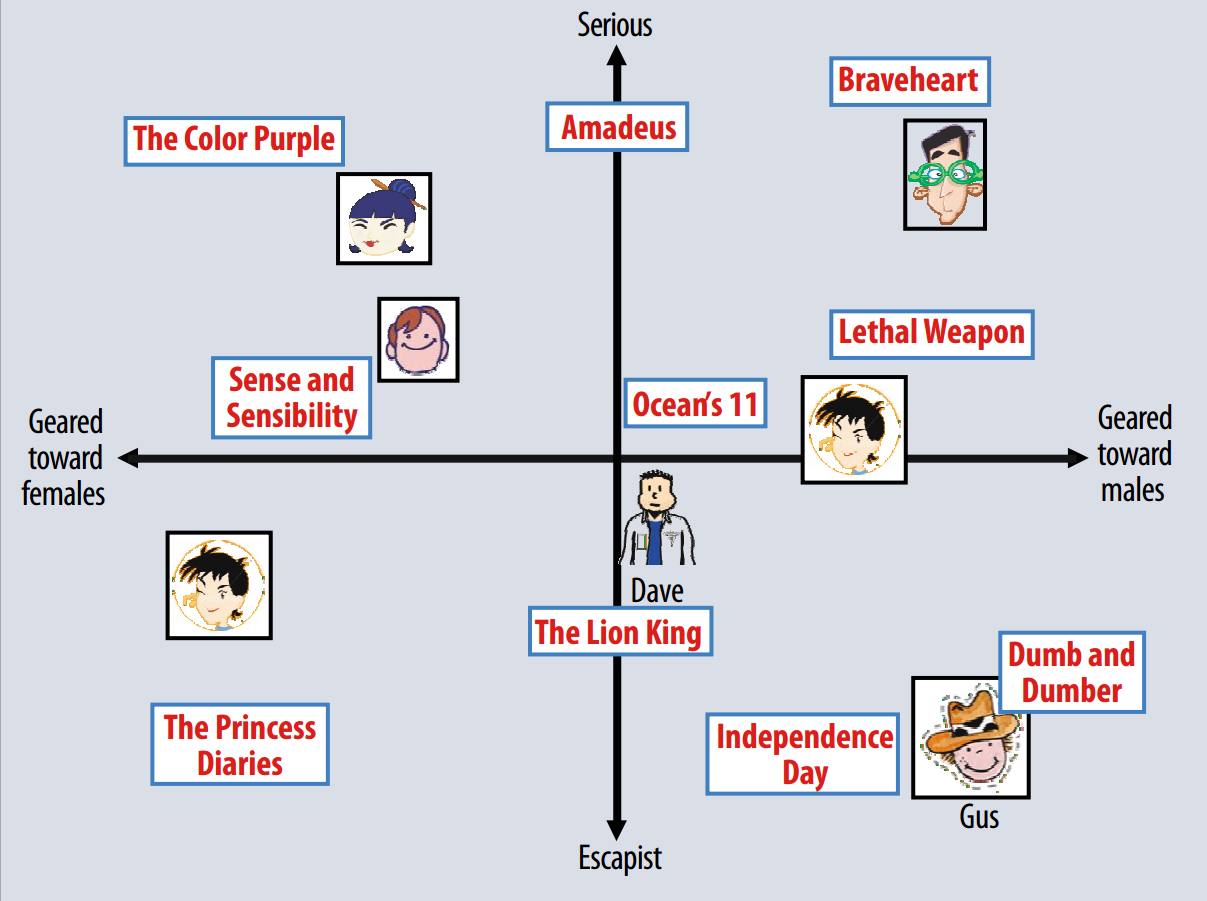
\includegraphics[height=5cm]{fig/factor_representation.png}
\caption{\label{nmet} A gauche : \textit{neighborhood methods}, A droite : \textit{Latent factor models}}
\end{center}
\end{figure}


\paragraph{\textit{Neighborhood methods}}




\paragraph{\textit{Latent factor model}}

\subsection{Factorisation de matrice}

\subsection{Notre approche et notations}

%% partie JB
%




\section{Algorithmes}

\subsection{Descente de gradient stochastique simple}

% Parler de la différence entre tirage avec remise ou sans. Quel est l'avantage théorique d'une descente de gradient sto?


\subsection{Algorithme parallélisé Jellyfish }





\section{Résultats}





\section*{Conclusion}

\newpage

\bibliographystyle{unsrt}
\bibliography{biblio}
\end{document}